\documentclass[11pt,a4paper]{article}

% --- Encoding & fonts ---------------------------------------------------------
\usepackage[utf8]{inputenc}
\usepackage[T1]{fontenc}
\usepackage{lmodern}
\usepackage{microtype}

% --- Geometry & layout --------------------------------------------------------
\usepackage[a4paper,margin=1in]{geometry}
\usepackage{setspace}
\setstretch{1.05}
\usepackage{parskip}
\usepackage{enumitem}
\setlist{nosep,leftmargin=1.4em}

% --- Typography ---------------------------------------------------------------
\usepackage{titlesec}
\titleformat{\section}{\large\bfseries}{\thesection.}{0.6em}{}
\titleformat{\subsection}{\normalsize\bfseries}{\thesubsection}{0.6em}{}
\usepackage{xcolor}
\definecolor{linkcol}{HTML}{1f4e79}
\definecolor{codebg}{HTML}{f2f2f2}
\definecolor{coderule}{HTML}{cccccc}

% --- Math, tables, figures ----------------------------------------------------
\usepackage{amsmath,amssymb}
\usepackage{booktabs}
\usepackage{array}
\usepackage{tabularx}
\usepackage{caption}
\captionsetup{font=small,labelfont=bf,skip=4pt}
\usepackage{graphicx}
\usepackage{float}

% --- Code listings ------------------------------------------------------------
\usepackage{listings}
\lstset{
  basicstyle=\ttfamily\footnotesize,
  backgroundcolor=\color{codebg},
  frame=single,
  framerule=0.4pt,
  rulecolor=\color{coderule},
  breaklines=true,
  columns=fullflexible,
  keepspaces=true,
  showstringspaces=false,
  xleftmargin=0.6em,
  xrightmargin=0.6em,
  aboveskip=6pt,
  belowskip=6pt
}

% --- TikZ ---------------------------------------------------------------------
\usepackage{tikz}
\usetikzlibrary{positioning,arrows.meta,shapes.geometric,fit,backgrounds,calc,shadows.blur}

% --- Hyperlinks (load near end) -----------------------------------------------
\usepackage[colorlinks=true,urlcolor=linkcol,citecolor=linkcol,linkcolor=linkcol]{hyperref}

% --- Bibliography -------------------------------------------------------------
\usepackage[numbers,sort&compress]{natbib}

% --- Title & authors ----------------------------------------------------------
\title{\textbf{java-codebase-rag}: A Graph-Native Code Intelligence Layer\\for Agentic Navigation of Java Microservice Codebases}

\author{
  Dmitriy Teriaev\thanks{Senior software engineer, Sberbank. Correspondence: \texttt{doudmitry@gmail.com}}
  \and
  Perplexity Computer\thanks{Co-author in the agentic-drafting sense: ideation, structure, prose, and diagrams were produced jointly with the human author over an extended design conversation.}
}

\date{May 2026}

\begin{document}
\maketitle

% =============================================================================
\begin{abstract}
\noindent
Large language model agents reason poorly about codebases the moment the codebase no longer fits in their context window. The standard remedy --- chunked retrieval-augmented generation over source files \cite{lewis2020rag} --- treats source code as prose and produces irrelevant or contradictory chunks for non-trivial questions ("who calls this method", "what HTTP routes does this microservice expose", "if I change this DTO, what breaks"). \textbf{java-codebase-rag} is a graph-native code intelligence layer that replaces chunk retrieval with deterministic graph navigation. It exposes a deliberately small Model Context Protocol (MCP) surface --- five tools: \texttt{search}, \texttt{find}, \texttt{describe}, \texttt{neighbors}, \texttt{resolve} --- backed by a typed property graph extracted from Java microservice source via tree-sitter \cite{treesitter}. The five tools collapse onto three primitive operations the agent actually performs: \emph{locate} a starting node (\texttt{search}, \texttt{find}, \texttt{resolve}); \emph{inspect} a node's full record (\texttt{describe}); \emph{walk} edges in the graph (\texttt{neighbors}). We call this metaphor \emph{a GPS for the agent}: the agent always knows where it is in the codebase, what is adjacent, and how to move. This report describes the architecture, the inspirations (GraphRAG \cite{edge2024graphrag}, the MCP standard \cite{anthropic2024mcp}, and the broader AST-graph-RAG line), and the design principles that shaped a v2 redesign from a 9-tool surface into the current 5-tool surface plus eight operator CLI subcommands grouped as lifecycle (\texttt{init}, \texttt{increment}, \texttt{reprocess}, \texttt{erase}), introspection (\texttt{meta}, \texttt{tables}, \texttt{diagnose-ignore}), and analysis (\texttt{analyze-pr}) (Section~\ref{sec:layer3} discusses the CLI briefly; full reference in \texttt{docs/JAVA-CODEBASE-RAG-CLI.md}). We do not include empirical evaluation: testing on real legacy codebases is in progress and the data is not yet ready to publish. The contribution of this report is conceptual: it argues for a particular shape of code-intelligence layer --- minimal, typed, graph-native, agent-shaped --- and shows the architecture in enough detail that a reader could rebuild it for another language ecosystem.
\end{abstract}

\vspace{0.6em}

% =============================================================================
\section{Frame: the agent needs a map, not a search engine}
\label{sec:frame}

Most code-intelligence systems that surface results to language models follow one of two patterns. \textbf{Pattern A: chunked RAG over source files} --- split source files into windowed chunks, embed, store in a vector database, retrieve the top-$k$ for any natural-language query, and inject the chunks into the prompt. This is the default RAG \cite{lewis2020rag} pattern transposed onto code, and it inherits all of RAG's failure modes: irrelevant chunks for structural queries, lost-in-the-middle effects \cite{liu2023lostmiddle} when several chunks must be reconciled, and silent omission of relevant code that didn't happen to embed near the query. \textbf{Pattern B: language-server bolted to a tool layer} --- expose a wide surface of LSP-style operations (find references, go to definition, list workspace symbols) as agent tools. This works for single-method questions but produces a sprawling tool catalog --- 20+ tools is common --- that weak models cannot navigate reliably and that contains pairs of redundant operations.

We argue for a third pattern. The agent does not need a search engine; the agent needs \emph{a map}. The map is a typed property graph extracted from the source. The agent's job is to navigate the map: pick a starting point, inspect what is there, walk to adjacent things. Three primitive operations are sufficient: \textbf{locate}, \textbf{inspect}, \textbf{walk}. Every realistic agent question over a codebase --- "who calls this", "what HTTP routes exist", "what DTOs cross this boundary", "if I change this method, what depends on it" --- decomposes into a chain of these three operations.

This is the GPS metaphor. The agent is always at some node in the graph. \texttt{search} and \texttt{find} get it to a starting node ("where am I?"). \texttt{describe} reports the full record at the current node ("what is here?"). \texttt{neighbors} returns adjacent nodes filtered by edge type and direction ("where can I go?"). The agent reasons; the system navigates. The agent does not retrieve text and reason about whether the text answers the question; it walks deterministic edges and reasons about the structure.

Reframing code intelligence as graph navigation has three immediate consequences. First, the tool surface shrinks dramatically and stops growing with new use cases --- new questions become new \emph{chains} of the existing tools, not new tools. Second, the system never returns "approximately relevant" results; every walk is exact (the edge either exists in the graph or it does not). Third, the failure mode shifts from "the model hallucinated" to "the graph is missing an edge type", which is a tractable engineering problem rather than a probabilistic one.

% =============================================================================
\section{Inspirations}
\label{sec:inspirations}

This system is not a research artefact. The architecture stitches together ideas from four streams of recent work; this section credits each.

\paragraph{GraphRAG and AST-graph retrieval.} Microsoft's GraphRAG \cite{edge2024graphrag} demonstrated that constructing a knowledge graph from source documents and retrieving over the graph --- with community detection for global summarisation and hierarchical context for local queries --- substantially outperforms flat vector retrieval for query-focused summarisation. The lesson generalises beyond text: \emph{any} corpus with strong relational structure benefits from extracting that structure once and querying it as a graph. Source code has the strongest relational structure of any corpus we routinely retrieve over (compilers extract it for free); not exploiting it is a missed opportunity. Subsequent work in the AST-graph-RAG line \cite{guo2024lightrag} reinforces the pattern: lighter, simpler graph backends with cleaner ontologies often beat heavyweight ones for retrieval quality.

\paragraph{Context engineering.} Context engineering --- filling the context window with the right information at the right time --- shaped our tool design. A tool that returns 5\,KB of plausibly-relevant text is not equivalent to a tool that returns 200 bytes of structured truth; the second is far more useful. Lost-in-the-middle effects \cite{liu2023lostmiddle} mean that long noisy contexts actively hurt downstream reasoning. The correct response is not "retrieve better" but "retrieve less, with type guarantees". Every tool in the java-codebase-rag surface returns small, typed, deterministic JSON. The agent never has to decide whether what it received is signal or noise.

\paragraph{Model Context Protocol.} The MCP standard \cite{anthropic2024mcp} fixed the impedance mismatch between agents and tools: a single transport, a single way to declare schemas, and a single way to bind tools to hosts (Claude Code, Cursor, Qwen Code, and others). Without MCP this report would describe a Claude-Code-only system. With MCP, a single Python server reaches every host the user already prefers. The standard does one thing well and stops.

\paragraph{The agent-skills layer.} Anthropic's agent skills \cite{anthropic2025skills} provided the missing piece between raw tool calls and agent reasoning: a skill is a slash-invokable, declaratively-described chain of tool calls that encodes a recurring intent ("trace this request flow", "show me callers of this method"). Skills are how a small fixed MCP surface grows into hundreds of usable agent intents without growing the tool count. Empirical testing showed that a single comprehensive skill (\texttt{/explore-codebase}) loaded at query time outperforms a large set of narrow per-intent skills, because the agent retains the full decision tree and recovery context rather than operating from a sliced subset.

\paragraph{What we are not.} We do not claim novelty over GraphRAG, LightRAG, or LSP-backed tooling. We claim that a particular synthesis --- minimal MCP surface, typed property graph, three-primitive navigation model, agent-shaped affordances --- is the right shape for code intelligence at the agentic-development layer. The synthesis is the contribution.

% =============================================================================
\section{Architecture: three layers}
\label{sec:architecture}

The system is organised in three layers (Figure~\ref{fig:layers}). Each layer has a single concern; layer boundaries are crossed only by typed contracts.

\begin{figure}[H]
\centering
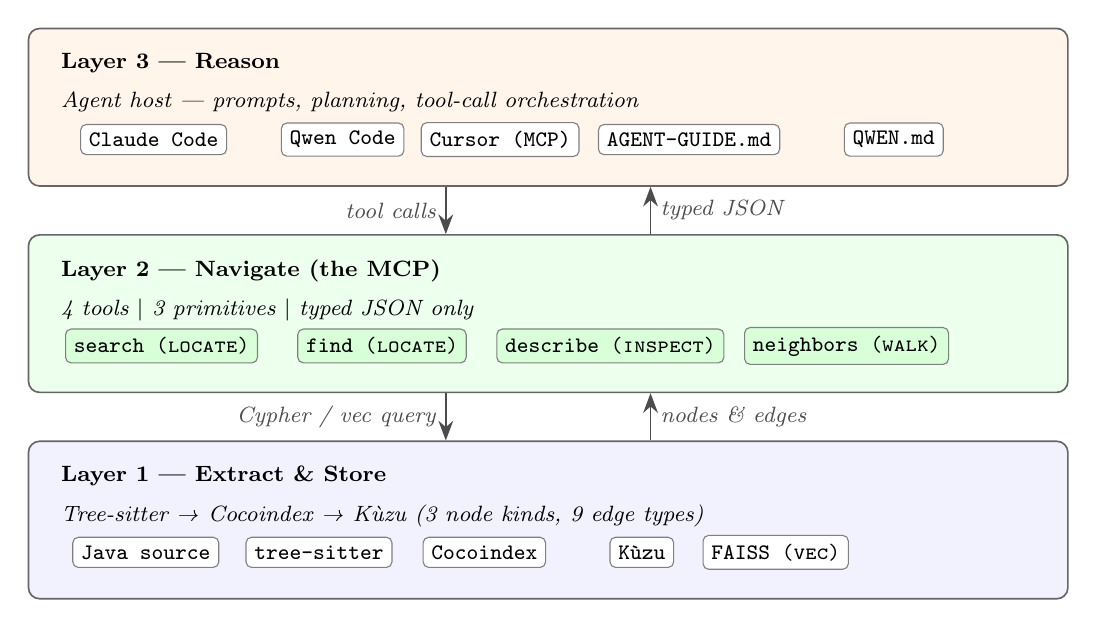
\begin{tikzpicture}[
  font=\small,
  node distance=0.6cm and 0.8cm,
  layer/.style={
    rectangle,
    rounded corners=4pt,
    draw=black!60,
    line width=0.6pt,
    minimum width=13.2cm,
    minimum height=2.0cm,
    align=left,
    inner sep=8pt
  },
  l1col/.style={fill=blue!5},
  l2col/.style={fill=green!7},
  l3col/.style={fill=orange!8},
  arrow/.style={-{Stealth[length=2.5mm]}, line width=0.6pt, black!70},
  pill/.style={
    rectangle, rounded corners=2pt,
    draw=black!50, fill=white, line width=0.4pt,
    inner sep=3pt, font=\footnotesize\ttfamily
  },
  label/.style={font=\footnotesize\bfseries, anchor=north west},
  sublabel/.style={font=\footnotesize\itshape, anchor=north west}
]

% --- Layer 3: Reason ---
\node[layer, l3col] (l3) {};
\node[label] at ($(l3.north west) + (0.3, -0.2)$) {Layer 3 \textemdash{} Reason};
\node[sublabel] at ($(l3.north west) + (0.3, -0.7)$) {Agent host \textemdash{} prompts, planning, tool-call orchestration};
\node[pill] at ($(l3.south west) + (1.6, 0.6)$) {Claude Code};
\node[pill] at ($(l3.south west) + (4.0, 0.6)$) {Qwen Code};
\node[pill] at ($(l3.south west) + (6.0, 0.6)$) {Cursor (MCP)};
\node[pill] at ($(l3.south west) + (8.4, 0.6)$) {AGENT-GUIDE.md};
\node[pill] at ($(l3.south west) + (11.0, 0.6)$) {QWEN.md};

% --- Layer 2: Navigate ---
\node[layer, l2col, below=of l3] (l2) {};
\node[label] at ($(l2.north west) + (0.3, -0.2)$) {Layer 2 \textemdash{} Navigate (the MCP)};
\node[sublabel] at ($(l2.north west) + (0.3, -0.7)$) {4 tools \textbar{} 3 primitives \textbar{} typed JSON only};
\node[pill, fill=green!15] at ($(l2.south west) + (1.7, 0.6)$) {search \textsc{(locate)}};
\node[pill, fill=green!15] at ($(l2.south west) + (4.5, 0.6)$) {find \textsc{(locate)}};
\node[pill, fill=green!15] at ($(l2.south west) + (7.4, 0.6)$) {describe \textsc{(inspect)}};
\node[pill, fill=green!15] at ($(l2.south west) + (10.4, 0.6)$) {neighbors \textsc{(walk)}};

% --- Layer 1: Extract & Store ---
\node[layer, l1col, below=of l2] (l1) {};
\node[label] at ($(l1.north west) + (0.3, -0.2)$) {Layer 1 \textemdash{} Extract \& Store};
\node[sublabel] at ($(l1.north west) + (0.3, -0.7)$) {Tree-sitter \textrightarrow{} Cocoindex \textrightarrow{} K\`uzu (3 node kinds, 9 edge types)};
\node[pill] at ($(l1.south west) + (1.5, 0.6)$) {Java source};
\node[pill] at ($(l1.south west) + (3.7, 0.6)$) {tree-sitter};
\node[pill] at ($(l1.south west) + (5.8, 0.6)$) {Cocoindex};
\node[pill] at ($(l1.south west) + (7.8, 0.6)$) {K\`uzu};
\node[pill] at ($(l1.south west) + (9.5, 0.6)$) {FAISS \textsc{(vec)}};

% --- Arrows: queries down, results up ---
\draw[arrow] ($(l3.south) + (-1.3,0)$) -- node[left, font=\footnotesize\itshape, pos=0.5] {tool calls} ($(l2.north) + (-1.3,0)$);
\draw[arrow] ($(l2.north) + (1.3,0)$) -- node[right, font=\footnotesize\itshape, pos=0.5] {typed JSON} ($(l3.south) + (1.3,0)$);

\draw[arrow] ($(l2.south) + (-1.3,0)$) -- node[left, font=\footnotesize\itshape, pos=0.5] {Cypher / vec query} ($(l1.north) + (-1.3,0)$);
\draw[arrow] ($(l1.north) + (1.3,0)$) -- node[right, font=\footnotesize\itshape, pos=0.5] {nodes \& edges} ($(l2.south) + (1.3,0)$);

\end{tikzpicture}

\caption{Three-layer architecture. \textbf{Layer 1 (Extract \& Store)} ingests Java source via tree-sitter and emits nodes and edges into an embedded property graph. \textbf{Layer 2 (Navigate)} exposes five MCP tools collapsing onto three primitive operations: locate, inspect, walk. \textbf{Layer 3 (Reason)} is the agent host (Claude Code, Qwen Code, or any MCP-compatible runtime) plus optional skills. Each layer is replaceable: swap the extractor for another language, swap the graph backend, swap the agent host --- contracts hold.}
\label{fig:layers}
\end{figure}

\subsection{Layer 1: extract and store}
\label{sec:layer1}

The extractor walks a Java source tree using tree-sitter \cite{treesitter} grammars. Tree-sitter gives an incremental, error-tolerant parse: the system handles syntactically-broken legacy code without aborting, which matters for the target environment (large Java microservice estates with ageing modules). The parser visits each declaration and emits typed graph nodes; a second pass resolves cross-file references and emits edges.

The graph is stored in K\`uzu \cite{kuzu2023}, an embedded property-graph database with a Cypher-style query language. K\`uzu was chosen over Neo4j for two pragmatic reasons: it embeds in-process (no separate database server to operate), and it has zero ongoing cost for a developer-side tool. Cocoindex \cite{cocoindex2024} drives the indexing pipeline (incremental rebuilds, dependency tracking, change detection on source files).

The ontology is small by design (Table~\ref{tab:ontology}). Three node kinds (\textsc{symbol}, \textsc{route}, \textsc{client}) cover everything an agent realistically asks about; ten edge types cover every relation we have found load-bearing in practice. The ontology version is currently 13; the discipline is that no edge type ships unless at least three realistic agent questions in our use-case backlog require it.

\begin{table}[H]
\centering
\small
\caption{The current ontology. Node kinds and edge types are deliberately few. The constraint is that every type pays for itself by enabling at least three concrete agent questions.}
\label{tab:ontology}
\begin{tabularx}{\textwidth}{l X}
\toprule
\textbf{Element} & \textbf{Description} \\
\midrule
\multicolumn{2}{l}{\emph{Node kinds}} \\
\textsc{symbol}  & A Java declaration: class, interface, enum, record, annotation, method, or constructor. The dominant node kind. \\
\textsc{route}   & An HTTP-exposed endpoint (Spring \texttt{@RequestMapping}, JAX-RS \texttt{@Path}, etc.). One per HTTP method + path. \\
\textsc{client}  & A typed reference to an external service: declared HTTP client (Feign, OpenFeign, REST clients) or messaging client. \\
\midrule
\multicolumn{2}{l}{\emph{Edge types (10)}} \\
\textsc{extends}        & Class- or interface-inheritance edge (Java \texttt{extends}). \\
\textsc{implements}     & Interface-implementation edge (Java \texttt{implements}). \\
\textsc{injects}        & Dependency-injection edge: a symbol receives another via constructor, field, or setter injection. \\
\textsc{overrides}      & Subtype method overrides a supertype declaration with the same signature. \\
\textsc{declares}       & Container declares a member: class \textsc{declares} method, package \textsc{declares} class, etc. \\
\textsc{declares\_client} & Module declares a typed external-service client. \\
\textsc{calls}          & In-process method call. The work-horse edge. \\
\textsc{exposes}        & A controller method \textsc{exposes} an HTTP route. \\
\textsc{http\_calls}    & Method invokes a declared HTTP client (cross-service edge). \\
\textsc{async\_calls}   & Method publishes to / consumes from a message broker (Kafka, RabbitMQ). \\
\bottomrule
\end{tabularx}
\end{table}

\subsection{Layer 2: navigate (the MCP)}
\label{sec:layer2}

Layer 2 is the public surface of the system. Five tools, three primitive operations (Figure~\ref{fig:gps}). Every tool returns small, typed JSON; no tool returns more than a single page of results without explicit pagination. Successful outputs may also carry advisory \texttt{hints} (templated next-call strings) and pagination echoes on \texttt{search} / \texttt{find}.

\begin{figure}[H]
\centering
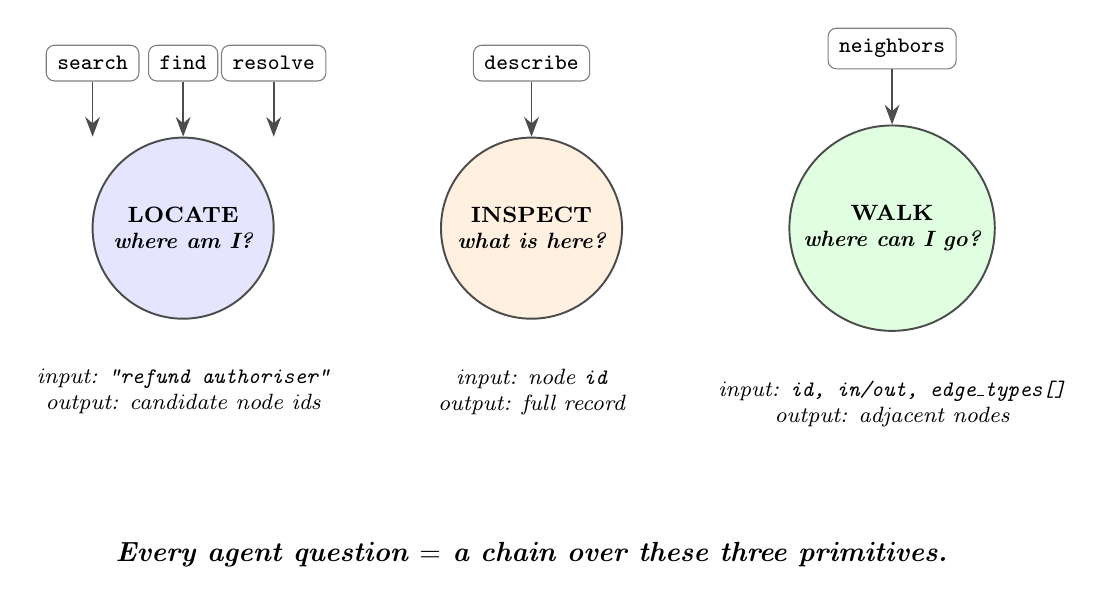
\begin{tikzpicture}[
  font=\small,
  node distance=1.3cm and 2.1cm,
  prim/.style={
    circle, draw=black!70, line width=0.7pt,
    minimum size=2.3cm, align=center,
    font=\footnotesize\bfseries
  },
  loc/.style={fill=blue!10},
  ins/.style={fill=orange!12},
  walk/.style={fill=green!12},
  tool/.style={
    rectangle, rounded corners=3pt,
    draw=black!50, fill=white, line width=0.4pt,
    inner sep=4pt, font=\footnotesize\ttfamily
  },
  arr/.style={-{Stealth[length=2.5mm]}, line width=0.6pt, black!70},
  q/.style={font=\footnotesize\itshape, align=center}
]

% --- Three primitives in a row ---
\node[prim, loc]  (locate)  {LOCATE\\ \footnotesize\itshape where am I?};
\node[prim, ins,  right=of locate] (inspect) {INSPECT\\ \footnotesize\itshape what is here?};
\node[prim, walk, right=of inspect] (walk)   {WALK\\ \footnotesize\itshape where can I go?};

% --- Tools above each primitive ---
\node[tool, above=0.7cm of locate, xshift=-1.15cm] (s)  {search};
\node[tool, above=0.7cm of locate, xshift=0cm]      (f)  {find};
\node[tool, above=0.7cm of locate, xshift=1.15cm]   (r)  {resolve};
\node[tool, above=0.7cm of inspect]                 (d)  {describe};
\node[tool, above=0.7cm of walk]                    (n)  {neighbors};

% --- Connections tools -> primitives ---
\draw[arr] (s)  -- (locate.north -| s);
\draw[arr] (f)  -- (locate.north -| f);
\draw[arr] (r)  -- (locate.north -| r);
\draw[arr] (d)  -- (inspect);
\draw[arr] (n)  -- (walk);

% --- Sample inputs/outputs below each primitive ---
\node[q, below=0.5cm of locate] (li) {input: \texttt{"refund authoriser"}\\ output: candidate node ids};
\node[q, below=0.5cm of inspect] (ii) {input: node \texttt{id}\\ output: full record};
\node[q, below=0.5cm of walk]    (wi) {input: \texttt{id, in/out, edge\_types[]}\\ output: adjacent nodes};

% --- Title strip below ---
\node[font=\itshape, below=2.7cm of inspect] (title)
  {\textbf{Every agent question $=$ a chain over these three primitives.}};

\end{tikzpicture}

\caption{The GPS metaphor. Five MCP tools collapse onto three primitive operations: \emph{locate} (where am I?), \emph{inspect} (what is here?), \emph{walk} (where can I go?). Every realistic agent question decomposes into a chain over these three primitives. The agent supplies the reasoning; the graph supplies the geometry.}
\label{fig:gps}
\end{figure}

\paragraph{\texttt{search} --- locate by meaning.} Semantic vector search over symbol descriptions, route paths, and client identifiers. Embeddings are produced by a sentence-BERT model \cite{reimers2019sbert}; the index is FAISS-backed \cite{johnson2019billion}. Returns ranked candidates with their \texttt{id}, \texttt{kind}, and a one-line summary. The agent uses \texttt{search} when it has a fuzzy starting query in natural language ("where do we authorise refund requests").

\paragraph{\texttt{find} --- locate by structure.} Filtered structured query over the graph. Takes a \texttt{kind} (\texttt{symbol}, \texttt{route}, or \texttt{client}) and a \texttt{NodeFilter} (15 optional fields: 3 universal, 5 symbol-specific, 3 route-specific, 4 client-specific). Returns deterministic, exhaustive results --- no ranking, no embeddings. The agent uses \texttt{find} when it knows the shape of what it wants ("all controller methods in the \texttt{auth} module exposed at \texttt{POST /authorise}").

\paragraph{\texttt{describe} --- inspect.} Returns the complete record for a single node by \texttt{id}, including all properties, the source file and line range, and a one-line summary. This is the only tool that returns more than identifiers and edge labels --- it is the agent's "zoom in" operation.

\paragraph{\texttt{neighbors} --- walk.} Graph traversal. Takes a node \texttt{id}, a \texttt{direction} (\texttt{in} or \texttt{out}), and a non-empty list of \texttt{edge\_types}. Returns adjacent nodes one hop away, optionally filtered by a \texttt{NodeFilter} on the destination. Multi-hop walks are explicit chains of \texttt{neighbors} calls --- the system never silently follows multiple hops, because that breaks the agent's ability to reason about what it just did.

The full type signatures are listed in Appendix~\ref{app:tools}. Two design choices in the current shape are worth surfacing:

\begin{enumerate}
\item \textbf{\texttt{NodeFilter} is one shared type, not three.} It has fields specific to symbol/route/client kinds, and the server validates that the filter is applicable to the queried kind. The alternative --- three separate filter types --- triples the schema surface for weak models with no expressive gain.
\item \textbf{Tool parameters are \texttt{Literal}-typed where finite.} \texttt{kind}, \texttt{direction}, \texttt{edge\_types}, and \texttt{symbol\_kind} all carry literal-string types in the schema, which gives weak models a closed enumeration to choose from. This was a v2.x improvement after observing weak models invent values like \texttt{kind="function"} in production traces.
\end{enumerate}

\subsection{Layer 3: reason (the agent)}
\label{sec:layer3}

Layer 3 is whatever MCP-compatible host the developer prefers --- Claude Code, Qwen Code, Cursor, or another runtime. The host loads the java-codebase-rag MCP server, sees the five tools, and the agent reasons over them. There is no logic in this layer that is specific to java-codebase-rag; the entire affordance is the five tools and a prose agent guide (\texttt{docs/AGENT-GUIDE.md}) that documents the canonical workflows --- forced reasoning preamble, decision tree, edge taxonomy, worked examples.

A single skill (\texttt{/explore-codebase}) wraps the full operating manual --- edge taxonomy, \texttt{NodeFilter} reference, decision tree, recovery playbook --- into one loadable prompt. Empirical testing on the target codebase showed that a comprehensive prose guide loaded as one skill outperforms a large set of narrow per-intent skills; the agent retains the full decision tree and recovery context rather than operating from a sliced subset.

% =============================================================================
\section{Agent workflow}
\label{sec:workflow}

Figure~\ref{fig:workflow} traces a representative interaction. The user asks "who calls \texttt{RefundService.approve}". The agent decomposes the question into three calls --- \texttt{search} to locate the candidate symbol, \texttt{describe} to confirm the right one, \texttt{neighbors(in, [CALLS])} to walk inbound call edges --- and reports the answer. The agent does not retrieve source files. The agent does not reason about whether retrieved chunks are relevant. The agent navigates.

\begin{figure}[!htbp]
\centering
\resizebox{\textwidth}{!}{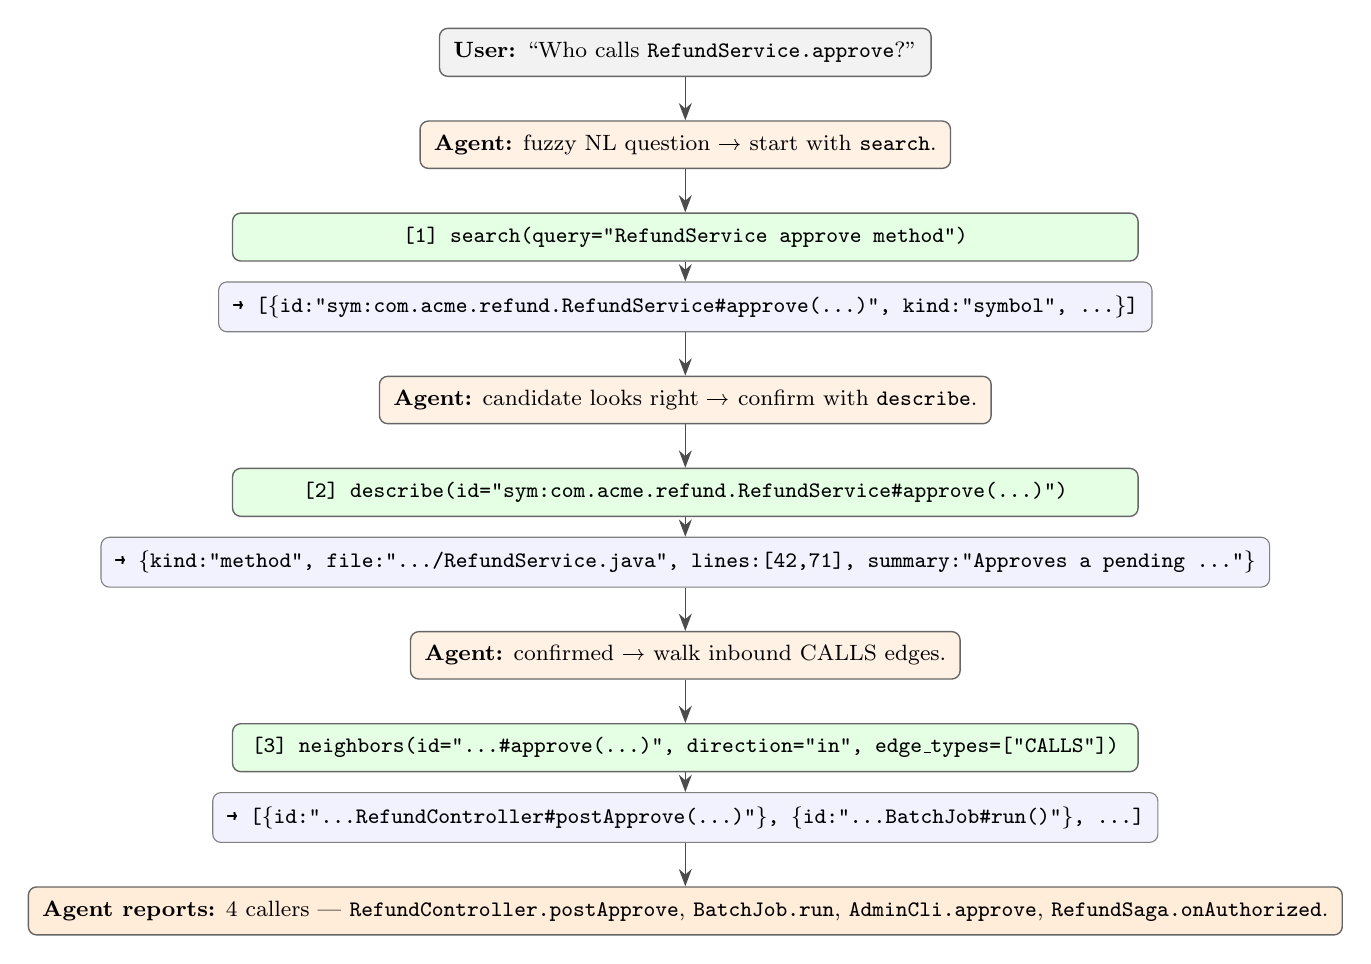
\begin{tikzpicture}[
  font=\footnotesize,
  node distance=0.55cm and 0.75cm,
  user/.style={
    rectangle, rounded corners=3pt, draw=black!60, fill=gray!10,
    line width=0.5pt, minimum width=4.5cm, align=left, inner sep=5pt
  },
  agent/.style={
    rectangle, rounded corners=3pt, draw=black!60, fill=orange!10,
    line width=0.5pt, minimum width=4.5cm, align=left, inner sep=5pt
  },
  call/.style={
    rectangle, rounded corners=3pt, draw=black!60, fill=green!10,
    line width=0.5pt, minimum width=11.5cm, align=left, inner sep=5pt,
    font=\footnotesize\ttfamily
  },
  result/.style={
    rectangle, rounded corners=3pt, draw=black!50, fill=blue!5,
    line width=0.4pt, minimum width=11.5cm, align=left, inner sep=5pt,
    font=\footnotesize\ttfamily
  },
  ans/.style={
    rectangle, rounded corners=3pt, draw=black!60, fill=orange!15,
    line width=0.5pt, minimum width=11.5cm, align=left, inner sep=5pt
  },
  arr/.style={-{Stealth[length=2.2mm]}, line width=0.4pt, black!70},
  lbl/.style={font=\footnotesize\bfseries\itshape}
]

% --- Step 0: user question ---
\node[user] (u) {\textbf{User:} ``Who calls \texttt{RefundService.approve}?''};

% --- Step 1: agent reasons ---
\node[agent, below=of u] (a1)
  {\textbf{Agent:} fuzzy NL question \textrightarrow{} start with \texttt{search}.};

% --- Call 1: search ---
\node[call, below=of a1] (c1)
  {[1] search(query="RefundService approve method")};
\node[result, below=0.25cm of c1] (r1)
  {\textrightarrow{} [\{id:"sym:com.acme.refund.RefundService\#approve(\ldots)", kind:"symbol", \ldots\}]};

% --- Step 2: agent confirms ---
\node[agent, below=of r1] (a2)
  {\textbf{Agent:} candidate looks right \textrightarrow{} confirm with \texttt{describe}.};

% --- Call 2: describe ---
\node[call, below=of a2] (c2)
  {[2] describe(id="sym:com.acme.refund.RefundService\#approve(\ldots)")};
\node[result, below=0.25cm of c2] (r2)
  {\textrightarrow{} \{kind:"method", file:"\ldots/RefundService.java", lines:[42,71], summary:"Approves a pending \ldots"\}};

% --- Step 3: agent walks ---
\node[agent, below=of r2] (a3)
  {\textbf{Agent:} confirmed \textrightarrow{} walk inbound CALLS edges.};

% --- Call 3: neighbors ---
\node[call, below=of a3] (c3)
  {[3] neighbors(id="\ldots\#approve(\ldots)", direction="in", edge\_types=["CALLS"])};
\node[result, below=0.25cm of c3] (r3)
  {\textrightarrow{} [\{id:"\ldots RefundController\#postApprove(\ldots)"\}, \{id:"\ldots BatchJob\#run()"\}, \ldots]};

% --- Final answer ---
\node[ans, below=of r3] (final)
  {\textbf{Agent reports:} 4 callers \textemdash{} \texttt{RefundController.postApprove}, \texttt{BatchJob.run}, \texttt{AdminCli.approve}, \texttt{RefundSaga.onAuthorized}.};

% --- Vertical arrows ---
\foreach \from/\to in {u/a1, a1/c1, c1/r1, r1/a2, a2/c2, c2/r2, r2/a3, a3/c3, c3/r3, r3/final}
  \draw[arr] (\from) -- (\to);

\end{tikzpicture}
}
\caption{A canonical agent interaction. Three tool calls, deterministic edges, typed JSON. Every step is auditable: the user can see exactly which graph edges were walked. There is no chunk retrieval; there is no scoring threshold to tune.}
\label{fig:workflow}
\end{figure}

The workflow is general. The java-codebase-rag agent guide enumerates 15+ canonical intents, each decomposing into 2--5 tool calls over the same five tools. New intents are new chains, not new tools.

A subtle point worth surfacing: the agent's first move is almost always \texttt{search}, not \texttt{find}. Natural-language questions arrive fuzzy; \texttt{search} is the cheapest way to get from "fuzzy English" to "candidate node ids". Once the agent has an id, all subsequent navigation is deterministic. This shape --- semantic at the boundary, structural in the interior --- is the practical reconciliation between vector retrieval and graph navigation. We do not need hybrid retrieval (parallel vector $+$ graph fusion) for most questions; we need \emph{sequential} retrieval, with the vector step strictly outside the graph step.

% =============================================================================
\section{Design principles}
\label{sec:principles}

The architecture above did not arrive in one step. It arrived after a v1 surface of nine MCP tools collapsed --- in design review --- into a small fixed set (currently five navigation tools). Five design principles guided the collapse, and they remain binding for any future surface change.

\begin{enumerate}
\item \textbf{The MCP is a graph navigator, not a reasoning engine.} If a tool's job is to combine results, summarise across nodes, or rank candidates, the tool belongs in the agent's reasoning, not the MCP. Move it to a skill or to a CLI subcommand.
\item \textbf{Every tool has a single primitive operation.} If a tool does two things ("search and describe", "find and walk"), it should be two tools or one tool with a strict contract. Composite tools confuse weak models and double the failure surface.
\item \textbf{Schemas are closed where finite.} Every parameter that takes one of $N$ known values is a \texttt{Literal}-typed enumeration. The agent gets explicit affordances; the server gets free input validation.
\item \textbf{Operational surface is human-shaped, not agent-shaped.} {\sloppy Tools the agent does not call belong in a CLI (\texttt{java-codebase-rag} lifecycle and introspection subcommands --- \texttt{init}, \texttt{increment}, \texttt{reprocess}, \texttt{erase}, \texttt{meta}, \texttt{tables}, \texttt{diagnose-ignore}, \texttt{analyze-pr}), not the MCP. The MCP navigation surface stays small and fixed; new agent intents are new chains over the existing tools, not new tools.\par}
\item \textbf{Walks are explicit, not silent.} The system never multi-hops without the agent asking. Multi-hop intents become multi-call chains. The agent always knows what edges it walked, and the user always can audit.
\end{enumerate}

The combined effect of these principles is that the MCP surface is provably small and grows slowly. It is allowed to add edge types (with the three-question rule), and it is allowed to refine schemas; it is not allowed to grow the tool count.

% =============================================================================
\section{What this deliberately does \emph{not} do}
\label{sec:nondoes}

A small system advertises its boundary. java-codebase-rag does not, and will not without a strong forcing function:

\begin{itemize}
\item \textbf{Generate code.} The agent's host already does this. java-codebase-rag is the navigation layer feeding the code-generating agent context; conflating roles destroys both.
\item \textbf{Track version-control history.} \texttt{git blame}, \texttt{who-changed-this}, ownership inference --- all out of scope until VCS data is modelled, which it currently is not.
\item \textbf{Cross language boundaries.} Java only. Polyglot support is a multi-PR effort that the current target environment does not need.
\item \textbf{Run hybrid retrieval} (parallel vector $\times$ graph fusion via reciprocal rank fusion or similar). The case for sequential retrieval (semantic at the boundary, structural inside) is strong; hybrid is research-only on the backlog.
\item \textbf{Summarise.} If the agent wants a summary, it asks the host model to summarise the deterministic JSON it just retrieved. java-codebase-rag never produces prose.
\end{itemize}

% =============================================================================
\section{Future work}
\label{sec:future}

{\sloppy
Three threads are open and prioritised. \textbf{(1) Real-codebase evaluation.} Testing on a large legacy Java microservice estate is in progress; once stable, we expect to publish accuracy numbers (intent $\to$ correct-tool-chain rate, end-to-end answer correctness against human labels) for the five-tool surface against weak (Qwen) and strong (Claude Sonnet 4.5) hosts. \textbf{(2) Lightweight skills.} A lightweight \texttt{/search-codebase} skill (search + find + shallow neighbors + host glob) is planned as a low-context-cost alternative to the comprehensive \texttt{/explore-codebase} skill for quick lookups. \textbf{(3) Tier-2 incremental rebuilds.} Today the index rebuilds the affected modules; we want commit-level incremental rebuilds for sub-second index updates on large monorepos.
\par}

We deliberately list \emph{no} item that would grow the MCP tool count without proof that the existing five tools cannot accommodate a real intent.

% =============================================================================
\section*{Acknowledgements}
This system was designed and built collaboratively over a long-running design conversation between the human author and Computer (Perplexity). Computer contributed the v2 collapse argument, the GPS framing, the schema-flattening fix for weak-model JSON encoding, and substantial portions of the prose in this report. The human author retained final design authority on every locked decision and ran every test.

% =============================================================================
\bibliographystyle{plainnat}
\bibliography{references}

% =============================================================================
\appendix
\section{Tool signatures (verbatim)}
\label{app:tools}

The five MCP tools have the following Python (Pydantic) signatures, simplified for readability. The full source lives at \texttt{mcp\_v2.py} in the repository.

\begin{lstlisting}[language=Python]
DeclarationSymbolKind = Literal[
    "class", "interface", "enum", "record",
    "annotation", "method", "constructor"
]

EdgeType = Literal[
    "EXTENDS", "IMPLEMENTS", "INJECTS", "OVERRIDES", "DECLARES",
    "DECLARES_CLIENT", "CALLS", "EXPOSES",
    "HTTP_CALLS", "ASYNC_CALLS"
]

class NodeFilter(BaseModel):
    # Universal
    microservice: str | None = None
    module: str | None = None
    name_contains: str | None = None
    # Symbol-specific
    symbol_kind: DeclarationSymbolKind | None = None
    symbol_kinds: list[DeclarationSymbolKind] | None = None
    fqn_contains: str | None = None
    role: str | None = None
    annotated_with: str | None = None
    # Route-specific
    http_method: str | None = None
    path_contains: str | None = None
    # Client-specific
    client_kind: str | None = None
    target_service: str | None = None

def search(query: str, limit: int = 25) -> list[NodeRef]: ...

def find(
    kind: Literal["symbol", "route", "client"],
    filter: NodeFilter | dict | str,
    limit: int = 25,
    offset: int = 0,
) -> FindOutput: ...

def describe(id: str) -> DescribeOutput: ...

def resolve(identifier: str, hint_kind: str | None = None) -> ResolveOutput: ...

def neighbors(
    id: str,
    direction: Literal["in", "out"],
    edge_types: list[EdgeType],  # min length 1
    filter: NodeFilter | dict | str | None = None,
    limit: int = 50,
) -> NeighborsOutput: ...
\end{lstlisting}

{\sloppy The CLI subcommands (\texttt{init}, \texttt{increment}, \texttt{reprocess}, \texttt{erase}, \texttt{meta}, \texttt{tables}, \texttt{diagnose-ignore}, \texttt{analyze-pr}) are documented separately in \texttt{docs/JAVA-CODEBASE-RAG-CLI.md} and are not part of the MCP surface.\par} Multi-agent considerations and host-collision behaviour are discussed in the linked design conversation; see also \cite{cognition2025multiagent}.

\end{document}
